% -----------------------------------------------
% Template for ISMIR Papers
% 2015 version, based on previous ISMIR templates
% -----------------------------------------------

\documentclass{article}
\usepackage{ismir,amsmath,cite}
\usepackage{graphicx}
\usepackage{color}
\usepackage{mathrsfs}
\usepackage[english]{babel}
\usepackage{caption}
\usepackage{subfig, color}

% Title.
% ------
\title{Learning invariants for polyphonic instrument recognition}


% Single address
% To use with only one author or several with the same address
% ---------------
%\oneauthor
% {Names should be omitted for double-blind reviewing}
% {Affiliations should be omitted for double-blind reviewing}

% Two addresses
% --------------
%\twoauthors
%  {First author} {School \\ Department}
%  {Second author} {Company \\ Address}

% Three addresses
% --------------
\threeauthors
  {First author} {Affiliation1 \\ {\tt author1@ismir.edu}}
  {Second author} {\bf Retain these fake authors in\\\bf submission to preserve the formatting}
  {Third author} {Affiliation3 \\ {\tt author3@ismir.edu}}

% Four addresses
% --------------
%\fourauthors
%  {First author} {Affiliation1 \\ {\tt author1@ismir.edu}}
%  {Second author}{Affiliation2 \\ {\tt author2@ismir.edu}}
%  {Third author} {Affiliation3 \\ {\tt author3@ismir.edu}}
%  {Fourth author} {Affiliation4 \\ {\tt author4@ismir.edu}}

\begin{document}
%
\maketitle
%
\begin{abstract}
The abstract should be placed at the top left column and should contain about 150-200 words.
\end{abstract}
%

\section{Introduction}\label{sec:introduction}
% audio vs symbolic levels of music information
% variability is dominated by melody and orchestration
% at the symbolic level, melodies are represented over a continuous pitch axis
% whereas instrument identities are categorical
% music instrument recognition is dual to music transcription

% the challenge is thus two-fold
% 1. gaining abstraction by integrating time-frequency patterns over longer time scales
% 2. building invariants to melody while remaining highly discriminative to the instrument



% On music instrument classification
% Ref to Joder et al
% Ref to Fuhrmann

% On feature learning
% Ref to Dieleman and Benjamin ICASSP 2014
% Ref to Humphrey, Bello, LeCun 2012
% Ref to Salamon and Bello
% Ref to Li, Qian, and Wang arXiv 2015

\section{Deep convolutional networks}
\subsection{Time-frequency representation}
We used the implementation from the librosa package \cite{McFee2015} with $Q=12$ filters per octave, center frequencies ranging from 55 Hz to 14 kHz (8 octaves from A1 to A9), and a hop size of 23 ms. Furthermore, we applied perceptual weighting of loudness in order to reduce the dynamic range between the fundamental partial and its upper harmonics. A 3-second sound excerpt $x(t)$ is represented by a time-frequency matrix $\boldsymbol{x_1}(t,k_1)$ of width $T=128$ samples and height $K_1=96$ MIDI indices.

\subsection{Architecture}
First of all, we apply a family $\boldsymbol{W_2}(\tau,\kappa_1,k_2)$ of $K_2=50$ learned time-frequency convolutional operators, whose supports are constrained to have width $\Delta t$ and height $\Delta k_1$. 

\begin{equation}
\boldsymbol{W_2}
\overset{t,k_1}{\ast}
\boldsymbol{x_1}
=
\! \!
\sum_{\substack{
0 \leq \tau < \Delta t \\
0 \leq \kappa_1 < \Delta k_1}} 
\! \! \! \! \!
\boldsymbol{W_2}(\tau,\kappa_1,k_2)
\boldsymbol{x_1}(t-\tau,k_1-\kappa_1)
\end{equation}

Furthermore, element-wise biases $\boldsymbol{b_2}(k_2)$ are added to the convolutions, resulting in the tensor 

\begin{equation}
\boldsymbol{y_2}(t,k_1,k_2) =
\boldsymbol{b_2} + 
(\boldsymbol{x_1}
\overset{t,k_1}{\ast}
\boldsymbol{W_2}).
\end{equation}
 
The second step is the application of a pointwise nonlinearity. We have chosen the \emph{rectified linear unit} (ReLU) because of its popularity in computer vision and its computational efficiency.
 
 \begin{equation}
 \boldsymbol{y_{2}^{+}}(t,k_1,k_2) = \max \left( \boldsymbol{y_2}(t,k_1,k_2), 0\right)
 \end{equation}
 
 To achieve invariance to translation as well as frequency transposition, we pool neighboring units in
 the time-frequency domain $(t,k_1)$ over non-overlapping rectangles of width $\Delta t$ and height $\Delta k_1$.
 
 \begin{equation}
 \boldsymbol{x_2}(t,k_1,k_2) =
 \max_{
\substack{
0 \leq \tau < \Delta t \\
0 \leq \kappa_1 < \Delta k_1}
 } \left\{
 \boldsymbol{y_{2}^{+}}(t + \tau, k_1 + \kappa_1, k_2)
 \right\}
 \end{equation}
 
 \begin{equation}
 \boldsymbol{y_3}(t,k_1,k_3) =
 \sum_{k_2}
 (\boldsymbol{x_2}
 \overset{t,k_1}{\ast}
 \boldsymbol{W_3})
 \end{equation}

\begin{equation}
\boldsymbol{x_4}(k_4) =
\left(
\sum_{v_3}
\boldsymbol{W_4}(k_4, v_3)
\boldsymbol{x_3}(v_3) \right)^{+}
\end{equation}

\begin{equation}
\boldsymbol{x_5}(k_5) =
\left(
\sum_{k_4}
\boldsymbol{W_5}(k_5, k_4)
\boldsymbol{x_4}(k_4)
\right)^{+}
\end{equation}

\begin{equation}
\boldsymbol{y_6}(k_6) =
\sum_{k_6}
\boldsymbol{W_6}(k_6,k_5)
\boldsymbol{x_5}(k_5)
\end{equation}

We define the categorical cross-entropy as

\begin{equation}
\mathscr{L}(\boldsymbol{x_6}, \mathcal{I}) =
- \sum_{k_5 \in \mathcal{I}} \log \sigma ( \boldsymbol{y_6}(k_6) ).
\end{equation}

The goal is to minimize the average loss $\mathscr{L}(\boldsymbol{x_6}, \mathcal{I})$ for across all pairs $(\boldsymbol{x_6}, \mathcal{I})$ in the training set.

\subsection{Training}
% Random crops
% Categorical cross-entropy
The network is trained on categorical cross-entropy over shuffled mini-batches of size 512 with uniform class distribution. The learning rate policy for each scalar weight in the network is  \emph{Adam} \cite{Kingma2015}, a state-of-the-art online optimizer for gradient-based learning.

% Adam optimizer
% Shuffled examples with uniform class distribution
% Mini-batch learning
% Dropout

\section{Deep supervision of melodic contour}
\subsection{Disentangling pitch from timbre}
% Source-filter equation
% Ref to LeCun on disentangling factors of variability
% Ref to deeply supervised nets
% Ref to NIPS 2015
% Ref to Mallat 2016

\subsection{Extraneous supervision}
% Equation that sums over k2
% Make a figure

\begin{equation}
\mathscr{L}(\boldsymbol{x_2}, \mathcal{P}) =
- \sum_{(t,k_1)\in\mathcal{P}} 
\log \sigma
\left( \sum_{k_2} \boldsymbol{x_2}(t,k_1,k_2) \right)
\end{equation}

\subsection{Joint supervision}
% Different equation
% Comment extraneous vs joint
% Visualization to compare learned filters


\section{Single-instrument classification}\label{sec:single-instrument}
\subsection{Experimental design}
In order to train the proposed algorithms, we used MedleyDB v1.1. \cite{Bittner2014}, a dataset of 122 multitracks annotated with instrument activations as well as melodic $f_0$ curves when present. We extracted the monophonic stems corresponding to a selection of eight pitched instruments (see Figure \ref{fig:instrument-distribution}. Stems with leaking instruments in the background were discarded. The resulting set was double-checked manually, and annotation mistakes were reported to MedleyDB curators for the next release.
The evaluation set consists of 120 recordings of solo music collected by Joder et al. \cite{Joder2009}. We discarded recordings with extended instrumental techniques, since they are under-represented in MedleyDB. Moreover, since the 

\begin{figure}[t]
    \begin{center}
        \setlength{\unitlength}{1cm}
        \begin{picture}(8,10.5)
        \put(0,0){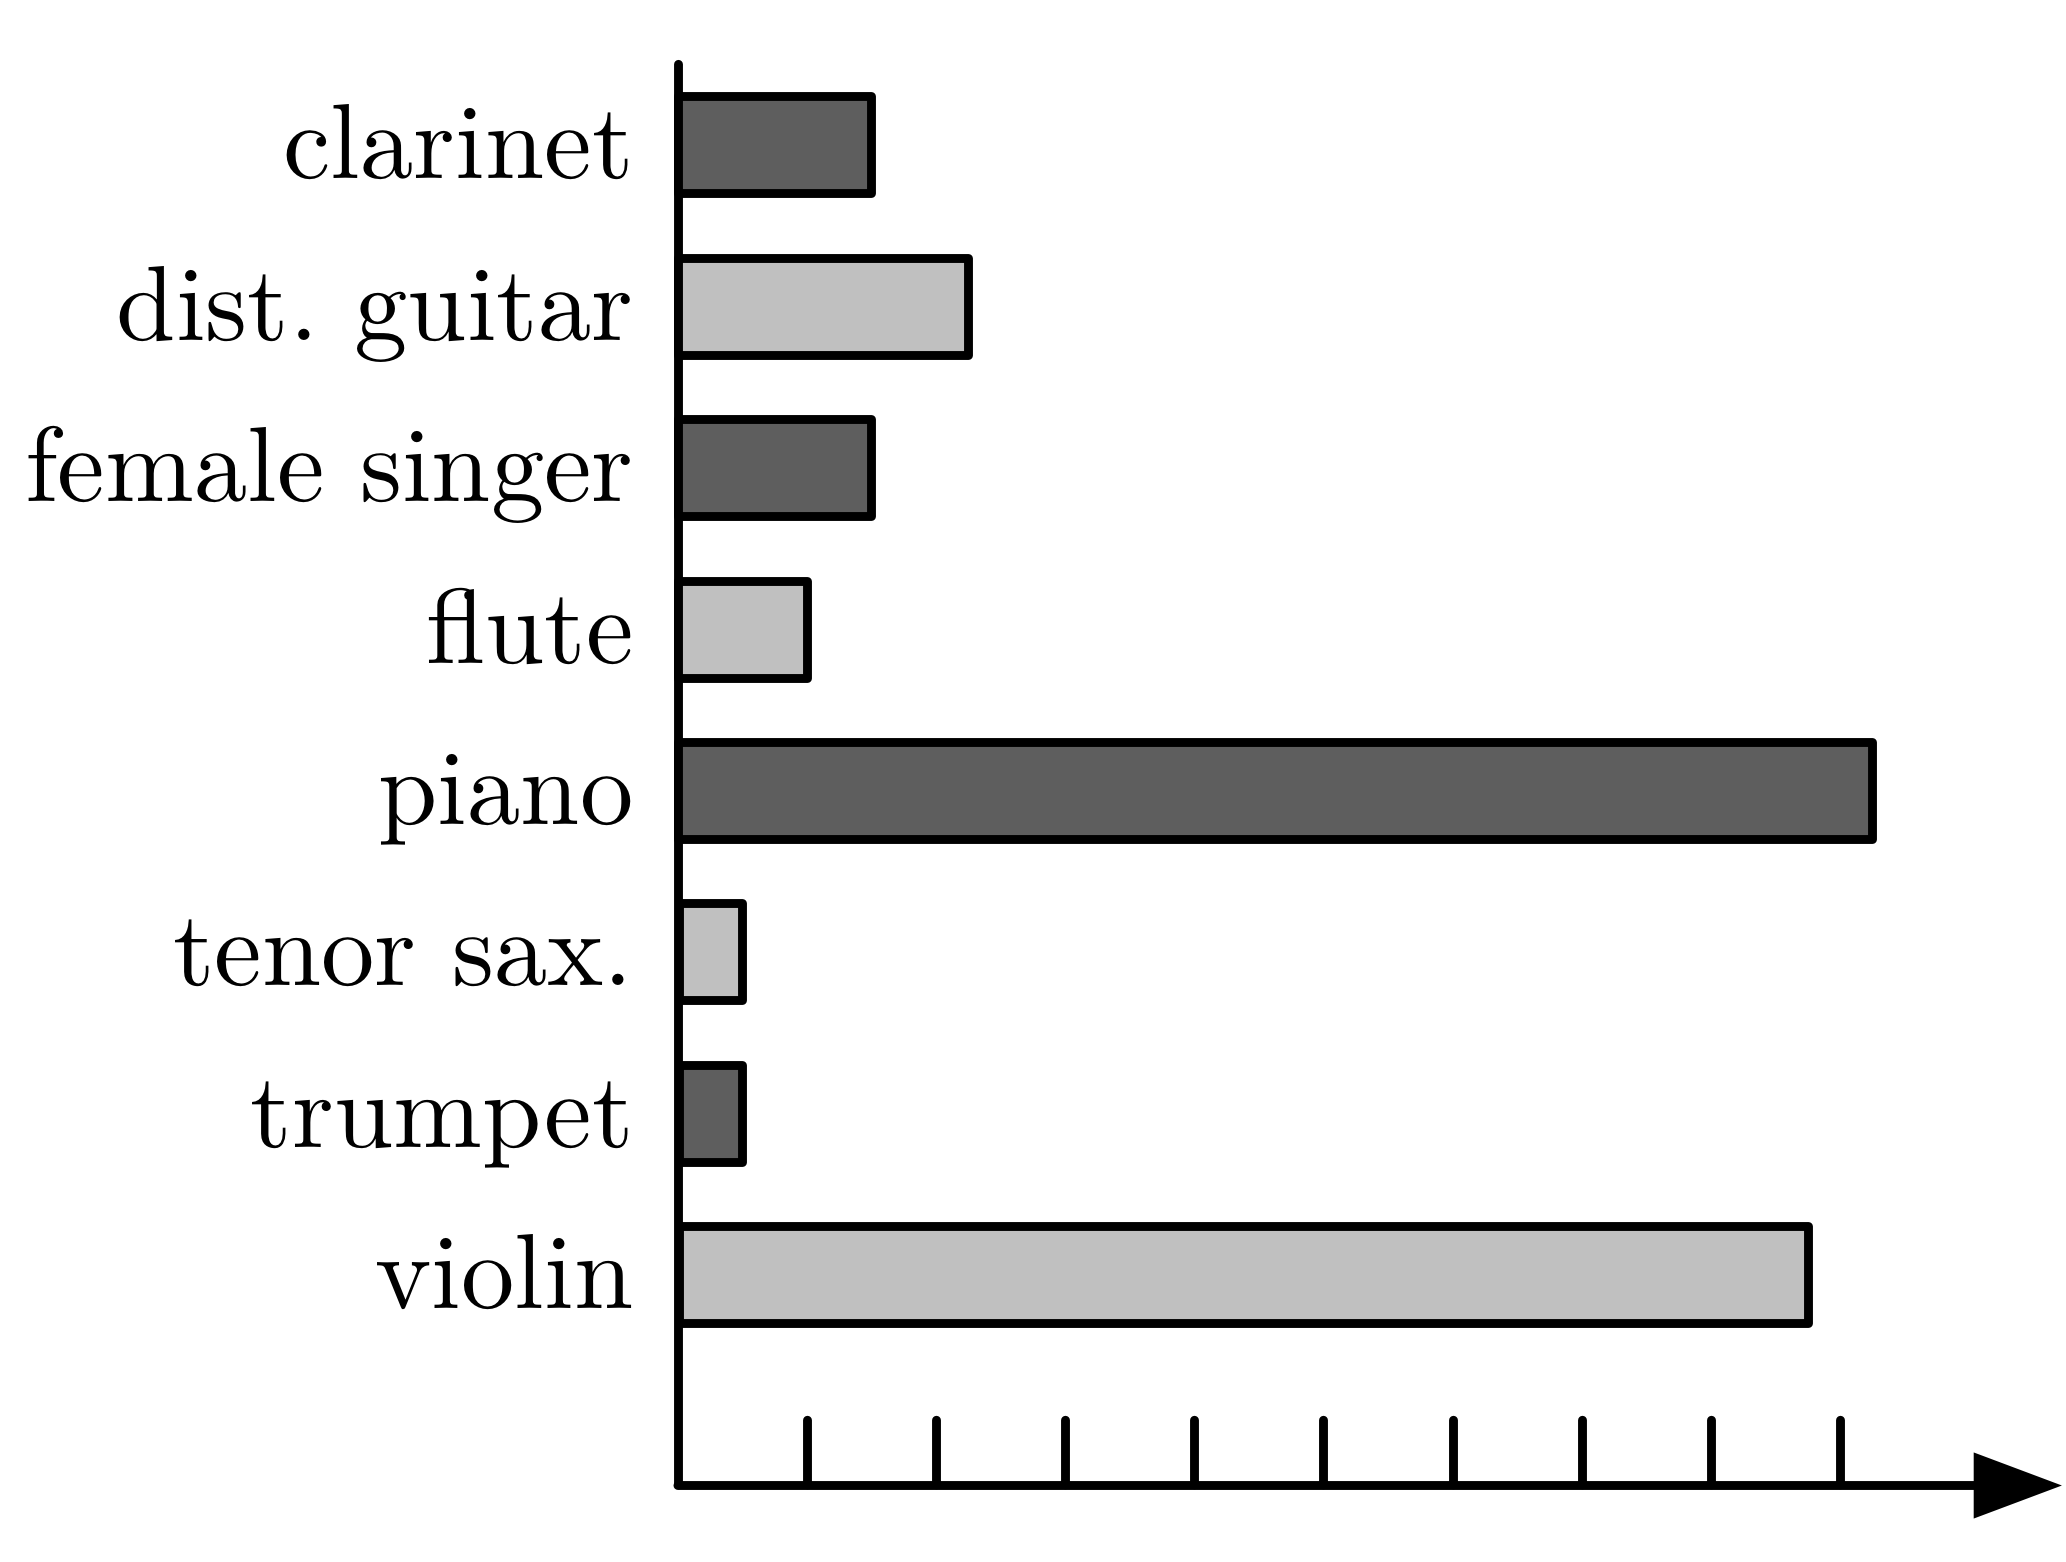
\includegraphics[width=8cm]{figs/distribution.png}}
        \end{picture}
    \end{center}
    \protect\caption{
    Amount of training data per instrument in MedleyDB, in minutes.
\label{fig:instrument-distribution}
}
\end{figure}

\subsection{Results}


\section{Polyphonic classification}\label{sec:polyphonic}
\subsection{Experimental design}

\subsection{Results}


\section{Conclusions}

% For bibtex users:
\bibliography{ISMIR2015template}

\end{document}
